\chapter{Evaluation}
\label{chap:eval}



\section{The Accuracy of the System}
\label{sec:eval-acc}

\subsection{Chinese Word Segmentation}
\label{ssec:eval-acc-chinese}

Tokenizing latin-script languages is not very hard. We can usually get by well
enough by splitting the text at whitespaces and at boundaries between different
classes of symbols. Sometimes, we might want to be more specific and try to
tokenize English contractions as separate words. However, these problems are
quite easy to solve when compared to the task of tokenizing Chinese text. The
absence of any spaces between words forbids the use of any simple heuristic and
linguistically empowered methods must be used.

We took inspiration from the system for Chinese word segmentation presented in
Section~\ref{survey-chinese} \cite{seg-chinese-maxent} which is also based on
maximum entropy models. The basic features used in that system were ported to
our formalism. The biggest difference between the systems was the fact that the
original Chinese tokenizer classified individual characters as being
single-character words or the beginning, middle or ending characters of a
multi-character word. However, the classifier used in our system is binary and
it decides for each character boundary whether it forms a token boundary or
not.

We were able to obtain the same data on which the original tokenizer was
developed, which happen to be the training data for the Second International
Chinese Word Segmentation Bakeoff \cite{web-bakeoff}. The bakeoff was a
competition challenging computational linguists to develop word segmentation
systems for Chinese using the supplied data for training. The provided data
consists of 4 datasets provided by Academia Sinica, City University of Hong
Kong, Peking University and Microsoft Research. Each of these datasets adopts
slightly different tokenization standards and so we train and test our
tokenizer on the datasets individually. Each dataset comes with a training part
and a testing part. We strictly used only the training part when developing our
tokenizer and used the testing part only at the end to evaluate our results.
The only thing we knew about the testing data in advance was its size which
helped us choose a reasonable size for our heldout data.

First off, we split our training data into a development part and a heldout
part. We chose the size of the heldout data to be roughly as big as the testing
data so we could trust our system's performance on it to be representative of
our system's true accuracy. The sizes of the partitioned datasets can be seen
in Table~\ref{tbl:bakeoff-sizes}.

\begin{table}
  \begin{center}
    \begin{tabular}{ | l | r | r | r | }
      \hline
      & \multicolumn{2}{ | c | }{Training data} & Testing data \\ \hline
      & Development data & Heldout data & Testing data \\ \hline
      Academia Sinica & 39686533 & 1057344 & 942571 \\ \hline
      City University & 8283540 & 266129 & 240767 \\ \hline
      Peking University & 7008808 & 719430 & 718331 \\ \hline
      Microsoft Research & 16100177 & 791333 & 766786 \\
      \hline
    \end{tabular}
  \end{center}
  \caption[Bakeoff dataset sizes]
    {The sizes of the individual parts of the bakeoff datasets in bytes.}
  \label{tbl:bakeoff-sizes}
\end{table}

We set the event cutoff to 2 as in \cite{seg-maxent-chinese}, so we retain a
lot of the encountered bigrams but still keep the number of parameters
manageable. We then experimented with training the tokenizer and testing it on
the heldout data. Depending on how much we constrained training time, the
tokenizer could either be undertrained or overfitted. The heldout data served
as an independent indicator telling us how close we are to the ideal balance
between a detailed and a general model. Experimentation led us to restrain the
number of training iterations to the values seen in
Table~\ref{tbl:bakeoff-iters}. We can see that the suitable number of
iterations spent training is nearly a linear function of the dataset size. This
stems from the fact that a larger dataset usually means more bigrams and
unigrams and thus more parameters to estimate.

\begin{table}
  \begin{center}
    \begin{tabular}{ | l | r | }
      \hline
      & Number of iterations \\ \hline
      Academia Sinica & 1000 \\ \hline
      City University & 175 \\ \hline
      Peking University & 150 \\ \hline
      Microsoft Research & 400 \\
      \hline
    \end{tabular}
  \end{center}
  \caption[Recommended iterations for Chinese segmentation]
    {A suitable number of iterations for training on a given dataset in the
     bakeoff data.}
  \label{tbl:bakeoff-iters}
\end{table}

After we established the training parameters, we trained the system on the
entire training data and checked its performance on the gold testing data. The
performance of the development system on the heldout data and of the final
system on the testing data can be seen in Tables \ref{tbl:bakeoff-devel} and
\ref{tbl:bakeoff-final}.

\begin{table}
  \begin{center}
    \begin{tabular}{ | l | r | r | r | r | }
      \hline
      & Accuracy & Precision & Recall & F-measure \\ \hline
      Academia Sinica & 95.55\% & 96.38\% & 95.78\% & 96.08\% \\ \hline
      City University & 91.58\% & 94.28\% & 91.67\% & 92.95\% \\ \hline
      Peking University & 92.70\% & 94.20\% & 93.70\% & 93.95\% \\ \hline
      Microsoft Research & 93.19\% & 95.71\% & 92.79\% & 94.22\% \\
      \hline
    \end{tabular}
  \end{center}
  \caption[Development performance of Chinese segmenter]
    {The performance of the system trained on the development data when
     tokenizing the heldout data.}
  \label{tbl:bakeoff-devel}
\end{table}

\begin{table}
  \begin{center}
    \begin{tabular}{ | l | r | r | r | r | }
      \hline
      & Accuracy & Precision & Recall & F-measure \\ \hline
      Academia Sinica & 93.82\% & 94.63\% & 94.92\% & 94.77\% \\ \hline
      City University & 91.75\% & 94.38\% & 91.62\% & 92.98\% \\ \hline
      Peking University & 91.94\% & 94.94\% & 91.43\% & 93.15\% \\ \hline
      Microsoft Research & 94.34\% & 96.19\% & 93.79\% & 94.98\% \\
      \hline
    \end{tabular}
  \end{center}
  \caption[Final performance of Chinese segmenter]
    {The performance of the system trained on the entire training data when
     tokenizing the gold testing data.}
  \label{tbl:bakeoff-final}
\end{table}

While the resulting adapted system does not perform as well as the original
word segmenter by Low, Ng and Guo \cite{seg-chinese-maxent}, it achieves a
median performance compared to the performance of the other bakeoff
submissions. The result is quite pleasing, given that the all we needed was to
write the feature definitions into a few files and toy with some training
parameters.

\subsection{Tokenization of Czech and English}
\label{ssec:eval-acc-eng}

For evaluating the accuracy of tokenizing Czech and English text, four
different methods were implemented. The Absolute Baseline relies on no other
piece of information than the current decision point and the whitespace
following it to classify boundaries. It is there to show the minimum possible
line every tokenizer should pass. The Simple Tokenizer checks for capital
letters before the period (initials) and after the period (start of a new
sentence). It represents the often too simple approach to tokenization. The
English-only Satz-like \cite{sbd-satz} system uses only part of speech data
about the surrounding tokens to predict a boundary. Finally, the Groomed
Tokenizer is the tokenization scheme used in the original reference
implementation, which has been supplied with lists of abbreviations and lots of
useful regular expressions.

All systems were tested both on a sample of data from CzEng and, in the case of
the English tests, also on the Brown corpus. All datasets were divided into
equally large development, heldout and testing sets to be used as in
Section~\label{ssec:eval-acc-chinese}. As for the part of speech data of the
Satz-like system, lexicons for each part of speech were extracted from the
training section of the Brown corpus for the Brown corpus exercise and from the
entire Brown corpus for the CzEng exercise. The results of the trials can be
seen on Tables~\ref{tbl:czeng-czseg}, \ref{tbl:czeng-cztok},
\ref{tbl:czeng-enseg}, \ref{tbl:czeng-entok}, \ref{tbl:brown-seg} and
\ref{tbl:brown-tok}.

\begin{table}
  \begin{center}
    \begin{tabular}{ | l | c | c | c | c | c | }
      \hline
      CzEng - Czech & \multicolumn{4}{ | c | }{Segmentation} \\ \hline
      & Acc. & Prec. & Rec. & F-m. \\ \hline
      Absolute Baseline & 78.08\% & 72.03\% & 98.87\% & 83.34\% \\ \hline
      Simple Tokenizer & 91.23\% & 90.27\% & 94.35\% & 92.27\% \\ \hline
      Groomed Tokenizer & 93.50\% & 91.74\% & 96.97\% & 94.29\% \\
      \hline
    \end{tabular}
  \end{center}
  \caption[Segmentation performance on Czech]
    {The sentence boundary disambiguiation performance of the various methods
     for tokenizing Czech on the CzEng sample.}
  \label{tbl:czeng-czseg}
\end{table}

\begin{table}
  \begin{center}
    \begin{tabular}{ | l | c | c | c | c | c | }
      \hline
      CzEng - Czech & \multicolumn{4}{ | c | }{Tokenization} \\ \hline
      & Acc. & Prec. & Rec. & F-m. \\ \hline
      Absolute Baseline & 98.92\% & 98.92\% & 100.00\% & 99.45\% \\ \hline
      Simple Tokenizer & 99.17\% & 99.17\% & 100.00\% & 99.58\% \\ \hline
      Groomed Tokenizer & 98.89\% & 98.89\% & 100.00\% & 99.44\% \\
      \hline
    \end{tabular}
  \end{center}
  \caption[Tokenization performance on Czech]
    {The token boundary disambiguiation performance of the various methods for
     tokenizing Czech on the CzEng sample.}
  \label{tbl:czeng-cztok}
\end{table}

\begin{table}
  \begin{center}
    \begin{tabular}{ | l | c | c | c | c | c | }
      \hline
      CzEng - English & \multicolumn{4}{ | c | }{Segmentation} \\ \hline
      & Acc. & Prec. & Rec. & F-m. \\ \hline
      Absolute Baseline & 82.20\% & 74.14\% & 99.81\% & 85.08\% \\ \hline
      Simple Tokenizer & 93.35\% & 90.41\% & 97.23\% & 93.70\% \\ \hline
      Satz-like System & 92.88\% & 91.92\% & 94.29\% & 93.09\% \\ \hline
      Groomed Tokenizer & 96.34\% & 94.21\% & 98.89\% & 96.49\% \\
      \hline
    \end{tabular}
  \end{center}
  \caption[Segmentation performance on English CzEng]
    {The sentence boundary disambiguiation performance of the various methods
     for tokenizing English on the CzEng sample.}
  \label{tbl:czeng-enseg}
\end{table}

\begin{table}
  \begin{center}
    \begin{tabular}{ | l | c | c | c | c | c | }
      \hline
      CzEng - English & \multicolumn{4}{ | c | }{Tokenization} \\ \hline
      & Acc. & Prec. & Rec. & F-m. \\ \hline
      Absolute Baseline & 97.14\% & 97.14 & 100.00\% & 98.54\% \\ \hline
      Simple Tokenizer & 99.18\% & 99.42\% & 99.73\% & 99.58\% \\ \hline
      Satz-like System & 99.33\% & 99.32\% & 100.00\% & 99.65\% \\ \hline
      Groomed Tokenizer & 99.03\% & 99.01\% & 100.00\% & 99.50\% \\
      \hline
    \end{tabular}
  \end{center}
  \caption[Tokenization performance on English CzEng]
    {The token boundary disambiguiation performance of the various methods for
     tokenizing English on the CzEng sample.}
  \label{tbl:czeng-entok}
\end{table}

\begin{table}
  \begin{center}
    \begin{tabular}{ | l | c | c | c | c | c | }
      \hline
      Brown & \multicolumn{4}{ | c | }{Segmentation} \\ \hline
      & Acc. & Prec. & Rec. & F-m. \\ \hline
      Absolute Baseline & 74.95\% & N/A & 0.0\% & N/A \\ \hline
      Simple Tokenizer & 99.33\% & 99.38\% & 98.03\% & 98.70\% \\ \hline
      Satz-like System & 99.50\% & 99.49\% & 98.54\% & 99.01\% \\ \hline
      Groomed Tokenizer & 99.49\% & 99.36\% & 98.59\% & 98.97\% \\
      \hline
    \end{tabular}
  \end{center}
  \caption[Segmentation performance on Brown]
    {The sentence boundary disambiguiation performance of the various methods
     for tokenizing English on the Brown corpus.}
  \label{tbl:brown-seg}
\end{table}

\begin{table}
  \begin{center}
    \begin{tabular}{ | l | c | c | c | c | c | }
      \hline
      Brown & \multicolumn{4}{ | c | }{Tokenization} \\ \hline
      & Acc. & Prec. & Rec. & F-m. \\ \hline
      Absolute Baseline & 88.27\% & 92.88 & 88.64\% & 90.71\% \\ \hline
      Simple Tokenizer & 98.80\% & 98.55\% & 99.59\% & 99.07\% \\ \hline
      Satz-like System & 98.97\% & 98.75\% & 99.67\% & 99.21\% \\ \hline
      Groomed Tokenizer & 99.75\% & 99.70\% & 99.91\% & 99.80\% \\
      \hline
    \end{tabular}
  \end{center}
  \caption[Tokenization performance on Brown]
    {The token boundary disambiguiation performance of the various methods for
     tokenizing English on the Brown corpus.}
  \label{tbl:brown-tok}
\end{table}

While the data from the CzEng dataset proves to be more difficult for all of
the participating tokenizers, the Satz-like system's segmentation performance
suffers the most. This was not unexpected as the Satz-like tokenizer relies on
a lexicon of part of speech tags extracted from parts of the Brown corpus. When
the tokenizer was evaluated on the Brown corpus, the lexicon was induced from
the training and heldout datasets. This gave the tokenizer's lexicon a 99.41\%
coverage on the training dataset and a 99.44\% coverage on the heldout dataset
(the coverage is not 100\% as some of the words containing dashes or
apostrophes were broken into separate rough tokens); the coverage on the
testing dataset was 95.75\%. On the other hand, when the tokenizer was
evaluated on the CzEng dataset, the coverage on the training, heldout and
testing datasets was 95.80\%, 95.95\% and 95.66\% respectively. This gives the
Satz-like tokenizer an advantage on the Brown corpus, where the training data
is used to its full potential.

The Simple Tokenizer offered quite a lot of performance for a little work.
However, when it comes to segmentation, the difference between the simple
features used by the Simple Tokenizer and the rich features in the Groomed
Tokenizer can show. The Simple Tokenizer also seems to have an affinity for
tokenization. This can be made use of by using one tokenizer with specific
features only for segmentation and then use another for tokenization or vice
versa.

The variations of the methods' performance can be also attributed to the great
difference between the two corpora. The difference can be seen by examining the
precision and recall of the Absolute Baseline. In the CzEng data, the majority of
the potential sentence boundary characters actually are sentence boundaries
whereas in the Brown corpus, 88.27\% of the potential sentence boundaries are
not sentence boundaries. The cause of this difference is most prominently the
fact that in the Brown corpus, a comma can sometimes end a sentence (such as in
poems). This also explains why the tokenizers score so high on the segmentation
of the Brown corpus.

\section{The Speed of the System}
\label{sec:eval-spd}

\begin{figure}
  \begin{center}
    % GNUPLOT: LaTeX picture with Postscript
\begingroup
  \makeatletter
  \providecommand\color[2][]{%
    \GenericError{(gnuplot) \space\space\space\@spaces}{%
      Package color not loaded in conjunction with
      terminal option `colourtext'%
    }{See the gnuplot documentation for explanation.%
    }{Either use 'blacktext' in gnuplot or load the package
      color.sty in LaTeX.}%
    \renewcommand\color[2][]{}%
  }%
  \providecommand\includegraphics[2][]{%
    \GenericError{(gnuplot) \space\space\space\@spaces}{%
      Package graphicx or graphics not loaded%
    }{See the gnuplot documentation for explanation.%
    }{The gnuplot epslatex terminal needs graphicx.sty or graphics.sty.}%
    \renewcommand\includegraphics[2][]{}%
  }%
  \providecommand\rotatebox[2]{#2}%
  \@ifundefined{ifGPcolor}{%
    \newif\ifGPcolor
    \GPcolorfalse
  }{}%
  \@ifundefined{ifGPblacktext}{%
    \newif\ifGPblacktext
    \GPblacktexttrue
  }{}%
  % define a \g@addto@macro without @ in the name:
  \let\gplgaddtomacro\g@addto@macro
  % define empty templates for all commands taking text:
  \gdef\gplbacktext{}%
  \gdef\gplfronttext{}%
  \makeatother
  \ifGPblacktext
    % no textcolor at all
    \def\colorrgb#1{}%
    \def\colorgray#1{}%
  \else
    % gray or color?
    \ifGPcolor
      \def\colorrgb#1{\color[rgb]{#1}}%
      \def\colorgray#1{\color[gray]{#1}}%
      \expandafter\def\csname LTw\endcsname{\color{white}}%
      \expandafter\def\csname LTb\endcsname{\color{black}}%
      \expandafter\def\csname LTa\endcsname{\color{black}}%
      \expandafter\def\csname LT0\endcsname{\color[rgb]{1,0,0}}%
      \expandafter\def\csname LT1\endcsname{\color[rgb]{0,1,0}}%
      \expandafter\def\csname LT2\endcsname{\color[rgb]{0,0,1}}%
      \expandafter\def\csname LT3\endcsname{\color[rgb]{1,0,1}}%
      \expandafter\def\csname LT4\endcsname{\color[rgb]{0,1,1}}%
      \expandafter\def\csname LT5\endcsname{\color[rgb]{1,1,0}}%
      \expandafter\def\csname LT6\endcsname{\color[rgb]{0,0,0}}%
      \expandafter\def\csname LT7\endcsname{\color[rgb]{1,0.3,0}}%
      \expandafter\def\csname LT8\endcsname{\color[rgb]{0.5,0.5,0.5}}%
    \else
      % gray
      \def\colorrgb#1{\color{black}}%
      \def\colorgray#1{\color[gray]{#1}}%
      \expandafter\def\csname LTw\endcsname{\color{white}}%
      \expandafter\def\csname LTb\endcsname{\color{black}}%
      \expandafter\def\csname LTa\endcsname{\color{black}}%
      \expandafter\def\csname LT0\endcsname{\color{black}}%
      \expandafter\def\csname LT1\endcsname{\color{black}}%
      \expandafter\def\csname LT2\endcsname{\color{black}}%
      \expandafter\def\csname LT3\endcsname{\color{black}}%
      \expandafter\def\csname LT4\endcsname{\color{black}}%
      \expandafter\def\csname LT5\endcsname{\color{black}}%
      \expandafter\def\csname LT6\endcsname{\color{black}}%
      \expandafter\def\csname LT7\endcsname{\color{black}}%
      \expandafter\def\csname LT8\endcsname{\color{black}}%
    \fi
  \fi
  \setlength{\unitlength}{0.0500bp}%
  \begin{picture}(7200.00,5040.00)%
    \gplgaddtomacro\gplbacktext{%
      \csname LTb\endcsname%
      \put(946,704){\makebox(0,0)[r]{\strut{} 0}}%
      \put(946,1383){\makebox(0,0)[r]{\strut{} 5}}%
      \put(946,2061){\makebox(0,0)[r]{\strut{} 10}}%
      \put(946,2740){\makebox(0,0)[r]{\strut{} 15}}%
      \put(946,3418){\makebox(0,0)[r]{\strut{} 20}}%
      \put(946,4097){\makebox(0,0)[r]{\strut{} 25}}%
      \put(946,4775){\makebox(0,0)[r]{\strut{} 30}}%
      \put(1078,484){\makebox(0,0){\strut{} 1}}%
      \put(1721,484){\makebox(0,0){\strut{} 2}}%
      \put(2365,484){\makebox(0,0){\strut{} 3}}%
      \put(3008,484){\makebox(0,0){\strut{} 4}}%
      \put(3652,484){\makebox(0,0){\strut{} 5}}%
      \put(4295,484){\makebox(0,0){\strut{} 6}}%
      \put(4939,484){\makebox(0,0){\strut{} 7}}%
      \put(5582,484){\makebox(0,0){\strut{} 8}}%
      \put(6226,484){\makebox(0,0){\strut{} 9}}%
      \put(6869,484){\makebox(0,0){\strut{} 10}}%
      \put(308,2739){\rotatebox{-270}{\makebox(0,0){\strut{}Seconds spent tokenizing the Brown corpus}}}%
      \put(3973,154){\makebox(0,0){\strut{}Maximum number of simultaneous work units}}%
    }%
    \gplgaddtomacro\gplfronttext{%
      \csname LTb\endcsname%
      \put(5882,4602){\makebox(0,0)[r]{\strut{}Groomed Tokenizer}}%
      \csname LTb\endcsname%
      \put(5882,4382){\makebox(0,0)[r]{\strut{}Satz-like Tokenizer}}%
      \csname LTb\endcsname%
      \put(5882,4162){\makebox(0,0)[r]{\strut{}Simple Tokenizer}}%
      \csname LTb\endcsname%
      \put(5882,3942){\makebox(0,0)[r]{\strut{}Baseline Tokenizer}}%
    }%
    \gplbacktext
    \put(0,0){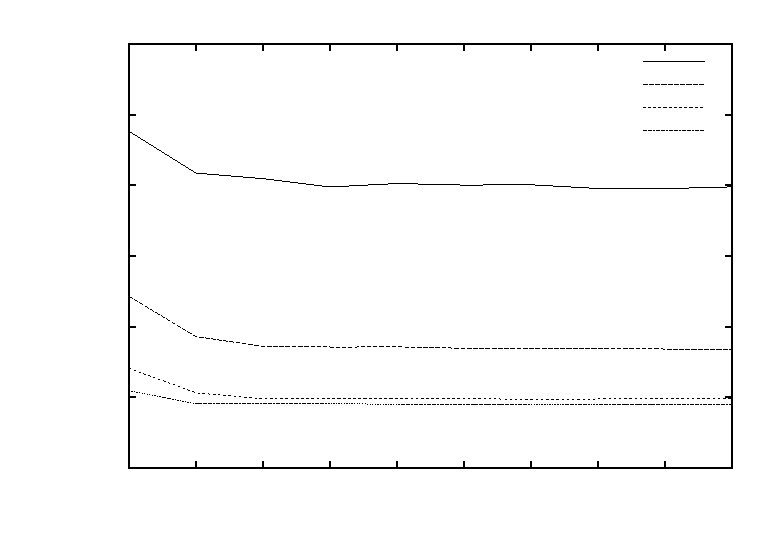
\includegraphics{img/work-units}}%
    \gplfronttext
  \end{picture}%
\endgroup

    \caption{The effect of maximum simultaneous work units on the performance of
             the tokenizer.}
    \label{fig:plot-work-units}
  \end{center}
\end{figure}
